\documentclass[11pt,a4paper]{article}
\usepackage[margin=2.3cm,headheight=15pt,headsep=9pt]{geometry}
\usepackage{graphicx}
\usepackage{booktabs}
\usepackage{amsmath,amssymb}
\usepackage{array}
\usepackage{xcolor}
\usepackage{tikz}
\usetikzlibrary{arrows.meta,positioning,fit,backgrounds,shapes.geometric}
\usepackage{caption}
\usepackage{pifont}
\usepackage[colorlinks=true,linkcolor=blue!50!black,citecolor=blue!50!black,
            urlcolor=blue!50!black]{hyperref}
\usepackage{lmodern}
\usepackage[expansion=false,final]{microtype}
\usepackage{titlesec}
\usepackage{fancyhdr}
\usepackage{enumitem}

\captionsetup{font=small,labelfont=bf,width=0.97\textwidth}
\titleformat{\section}{\large\bfseries}{\thesection}{0.7em}{}
\titleformat{\subsection}{\normalsize\bfseries}{\thesubsection}{0.6em}{}
\setlist{nosep,leftmargin=1.3em}
\pagestyle{fancy}\fancyhf{}
\fancyhead[L]{\footnotesize FlyScale: geometric scaling of the adult \textit{Drosophila} connectome}
\fancyhead[R]{\footnotesize\thepage}
\renewcommand{\headrulewidth}{0.3pt}
\setlength{\parskip}{0.35em}
\newcommand{\code}[1]{\texttt{\footnotesize #1}}
\newcommand{\gaa}{$G_1$}

\begin{document}
\sloppy


% ===================================================================== cover
\thispagestyle{empty}
\begin{tikzpicture}[remember picture,overlay]
  \node[inner sep=0pt] at (current page.center)
    {\includegraphics[width=\paperwidth,height=\paperheight]{figs/fig\_cover.pdf}};
\end{tikzpicture}
\clearpage

% ===================================================================== title
\thispagestyle{empty}
\begin{center}
{\LARGE\bfseries FlyScale: geometric scaling of the\\[0.15em]
adult \textit{Drosophila} connectome\par}
\vspace{0.7em}
{\large Structure, dynamics, capability and energy across a 10$\times$ ladder\par}
\vspace{0.9em}
{\normalsize Rick Goldberg\par}
{\footnotesize built and executed with an autonomous agent harness (\code{hermes-agent})\par}
\vspace{0.5em}
{\footnotesize Project repository: \code{\textasciitilde/Projects/VybFly}\quad$\cdot$\quad
all artifacts cited by path in Appendix~B\par}
\vspace{1.1em}
\end{center}

\begin{abstract}
\noindent
Can a biological connectome be enlarged? We take the complete adult \textit{Drosophila}
connectome (FlyWire FAFB v783; 139{,}255 neurons, 2{,}700{,}513 thresholded connections,
34{,}153{,}566 synapses) and ask whether a synthetic graph can be generated that preserves its
structural statistics, its propagation dynamics, its behavioural capabilities and its energy
budget as it grows. The method is a geometric one. We first fit latent coordinates to the
connectome and ask which space actually predicts connectivity: a 32-dimensional spectral
embedding predicts held-out connections best (AUC 0.952), a 2-D hyperbolic embedding beats the
anatomical 3-D soma coordinates (0.865 vs 0.851), and no embedding beats a degree-only baseline
by a margin larger than its own run-to-run spread. Scaling then proceeds by node subdivision in
that geometry: each neuron is replaced by $c$ children placed near it, each inheriting the
parent's partner set and synapse weights, with the concrete target chosen by the fitted
connection law $P(\text{connect}\mid \text{distance}) = 1/(1+e^{(d-R)/T})$. The result is a
ladder of graphs at $2\times$, $5\times$ and $10\times$ (up to 1{,}392{,}550 neurons and 27.8M
connections) whose connection count scales as $N^{1.0175}$ ($R^2=0.9995$) --- sparsity is
preserved, mean degree and mean connection strength stay bounded --- and which renormalizes back
to the biological graph almost exactly ($R(G_{10})$ returns 2{,}700{,}513 connections with a
degree-distribution distance of 0 and community ARI 1.0). Capability grows on some axes
(stimulus-discrimination information $\propto N^{1.014}$, participation ratio $\propto
N^{0.318}$, memory capacity $\geq 96$ associations versus 8 at $1\times$) and is flat on others
(temporal depth and sequence depth never rise above chance at any scale). An associative-learning
benchmark on the real mushroom body acquires odour--reward associations (AUC $0.51\to1.00$ in 58
trials) but the connectome's specific wiring contributes \emph{nothing} beyond shuffled controls
($+0.000\pm0.000$): what matters is the dopamine-gating anatomy, not the geometry. Energy is
measured on two tracks that are never summed: hardware (438/500/946/2022 GPU joules across the
ladder, with cost per spike \emph{falling} from 8.9 to 4.2~$\mu$J as the device stops being
launch-bound) and biological-equivalent ($P_{\text{bio}} = P_0 N/N_0$ from nanowatt calorimetry,
a property of $N$ alone). The work is deliberately dual-implementation: a Python reference oracle
and a Vyb-native production path (loader, discrete-event runtime, GPU kernels), and the effort to
build the second one surfaced twelve compiler defects, of which the blocking one --- a
kernel-mode store that wrote eight bytes into a four-byte slot --- is documented, fixed upstream
and verified here. We report what failed as carefully as what worked: a closure test that
demonstrates invertibility rather than self-similarity, a capability curve censored at its test
grid, a geometry that helps prediction but not renormalization, and a GPU backend whose
equivalence to the CPU reference had to survive two independent bugs, one of them ours.
\end{abstract}

\vspace{0.6em}
\begin{center}
\small
\begin{tabular}{ll}
\toprule
verdict (criterion \S25 of the project brief) & \\
\midrule
minimum success & \textbf{supported} \\
strong success & \textbf{supported} \\
exceptional ($C(N)$ growing faster than $P(N)$) & \textbf{not supported} \\
\bottomrule
\end{tabular}
\end{center}

\clearpage
\setcounter{page}{1}

% ===================================================================== 1
\section{Introduction and concept}
\label{sec:intro}

The whole-brain connectome of an adult female \textit{Drosophila} is the first complete wiring
diagram of a brain at synapse resolution~\cite{flywire-flagship,flywire-network}. It contains
$\approx$139k neurons and $\approx$54.5M synapses (16.8M directed neuron pairs before
thresholding), and it is not a random graph: it is sparse (connection probability
$\approx1.4\times10^{-4}$), weighted (a typical connection carries 12.6 synapses), organised into
79 neuropils, rich-club dominated (30\% of neurons are highly connected), and heavy-tailed in
degree~\cite{flywire-network}. It is, in short, exactly the kind of object for which a question
about \emph{scale} is well posed: if this graph is the product of biological growth rules, is
there enough structure in it to regenerate a larger one that still behaves like a brain?

This paper reports an attempt to answer that empirically, and the answer is deliberately split.
The machinery works: we can build a $10\times$ graph (1.39M neurons, 27.8M connections) that
preserves sparsity, degree distribution, community structure and propagation dynamics, and that
renormalizes back to the biological graph essentially exactly. Capability grows on the axes one
would expect from sheer size (information, dimensionality, associative capacity) and does not
grow on the axes that require temporal machinery (delay, sequence). And when we test the
connectome's own structure against shuffled controls in a learning task, the structure
contributes nothing measurable --- a negative result we regard as one of the more useful
findings here, because it constrains what "the connectome is special" can mean.

\paragraph{Concept.} The hypothesis under test is geometric, following the renormalization
programme for complex networks~\cite{geom-renorm}: real networks embedded in a hidden metric
space can be renormalized by rescaling distances, and networks with scale-free degree
distributions show geometric scaling under that transformation. The programme suggests a
concrete recipe: (i) fit a latent geometry to the graph; (ii) fit the connection law that
relates distance to connection probability; (iii) \emph{coarse-grain} by grouping nodes that are
close in that geometry (downscaling); (iv) \emph{subdivide} nodes and rewire by the same law
(upscaling); (v) accept the result only if the generated graph, coarse-grained back, recovers the
original. Step (v) is the crux, and we treat it as the primary acceptance criterion rather than a
sanity check.

Figure~\ref{fig:concept} lays out the object of study: one biological graph at the centre, a
downscaling branch to the left, an upscaling ladder to the right, and the closure loop that
decides whether the right-hand branch is legitimate. Every number on that diagram is a measured
value from this project.

\begin{figure}[t]
\centering
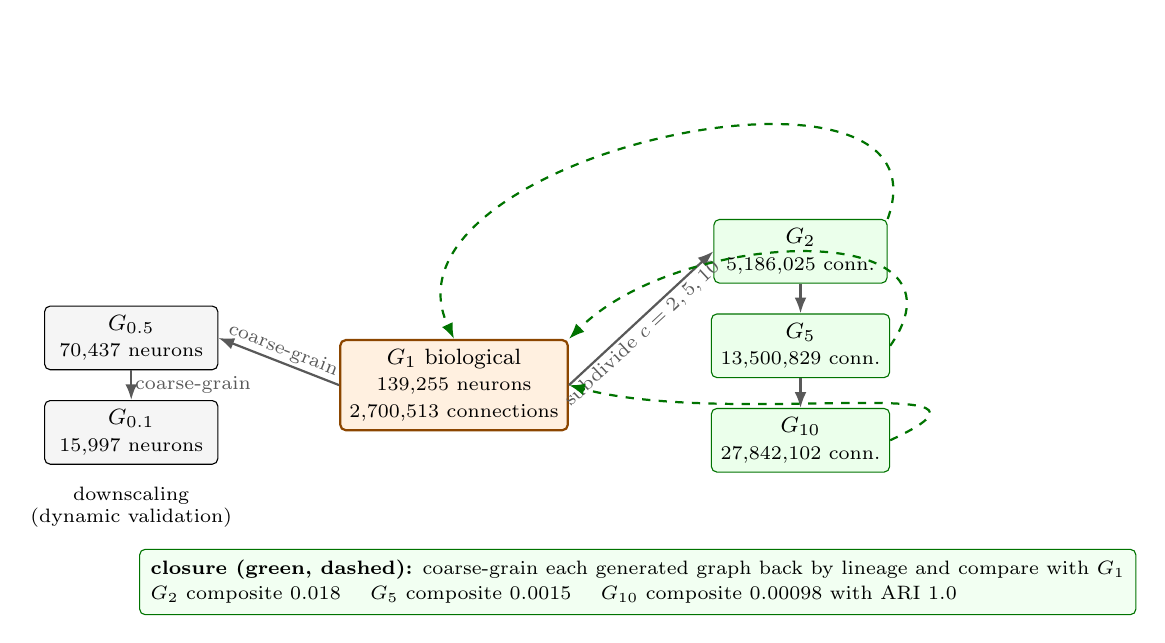
\begin{tikzpicture}[
  gnode/.style={draw,rounded corners=2pt,minimum width=2.2cm,minimum height=0.8cm,
                align=center,font=\footnotesize,fill=blue!4},
  bio/.style={gnode,fill=orange!12,draw=orange!55!black,thick},
  ok/.style={gnode,fill=green!8,draw=green!45!black},
  small/.style={gnode,fill=gray!8},
  ar/.style={-{Latex[length=2mm]},thick,gray!70!black},
  cl/.style={-{Latex[length=2mm]},thick,dashed,green!45!black},
  lab/.style={font=\scriptsize,inner sep=1pt}
]
% downscaling branch
\node[small] (g05) at (0,1.15) {$G_{0.5}$\\\scriptsize 70{,}437 neurons};
\node[small] (g01) at (0,-0.05) {$G_{0.1}$\\\scriptsize 15{,}997 neurons};
\draw[ar] (g05) -- node[lab,right]{coarse-grain} (g01);
\node[lab,align=center] at (0,-1.0) {downscaling\\(dynamic validation)};
% biological reference
\node[bio] (g1) at (4.1,0.55) {$G_1$ biological\\\scriptsize 139{,}255 neurons\\\scriptsize 2{,}700{,}513 connections};
\draw[ar] (g1.west) -- node[lab,above,sloped]{coarse-grain} (g05.east);
% upscaling ladder
\node[ok] (g2) at (8.5,2.25) {$G_2$\\\scriptsize 5{,}186{,}025 conn.};
\node[ok] (g5) at (8.5,1.05) {$G_5$\\\scriptsize 13{,}500{,}829 conn.};
\node[ok] (g10) at (8.5,-0.15) {$G_{10}$\\\scriptsize 27{,}842{,}102 conn.};
\draw[ar] (g2) -- (g5);
\draw[ar] (g5) -- (g10);
\draw[ar] (g1.east) -- node[lab,below,sloped,pos=0.45]{subdivide $c=2,5,10$} (g2.west);
% closure loop: arcs carry no labels, the legend below carries the numbers
\draw[cl] (g2.north east) to[out=70,in=115,looseness=1.15] (g1.north);
\draw[cl] (g5.east) to[out=55,in=45,looseness=1.25] (g1.north east);
\draw[cl] (g10.east) to[out=25,in=-15,looseness=1.3] (g1.east);
\node[draw,rounded corners=2pt,fill=green!5,draw=green!45!black,align=left,
      font=\scriptsize,inner sep=4pt,anchor=west] at (0.1,-1.95)
  {\textbf{closure (green, dashed):} coarse-grain each generated graph back by lineage and compare with $G_1$\\[1pt]
   $G_2$ composite $0.018$ \quad $G_5$ composite $0.0015$ \quad $G_{10}$ composite $0.00098$ with ARI $1.0$};
\end{tikzpicture}
\caption{The concept, with measured values. The biological graph \gaa{} is reproduced from the
FlyWire v783 release at a five-synapse threshold. Downscaling (coarse-graining in a latent
geometry) produces smaller replicas used to test whether dynamics survive compression; upscaling
(node subdivision guided by the fitted connection law) produces the ladder that is the subject of
the paper. The dashed green loop is the closure criterion: each generated graph is coarse-grained
back by lineage and compared with \gaa{} across a metric suite. Boxes show the measured
connection counts and closure composites (\S\ref{sec:scaling}); the $10\times$ graph returns the
biological connection count exactly.}
\label{fig:concept}
\end{figure}

\paragraph{Why this is not a neural-network paper.} The brief this project follows forbids
claiming consciousness, mapping the connectome onto transformers, pretending synapse counts are
learned weights, or inferring biological efficiency from GPU power numbers. The findings below
are correspondingly narrow: they are statements about a graph, a simulator and a
power meter. Where the evidence is a model identity rather than a measurement (the biological
energy track is linear in $N$ by construction) we say so in the same sentence that reports it.

\paragraph{Contributions.}
\begin{enumerate}[label=\textbf{C\arabic*.}]
\item A reproducible canonical dataset from the v783 release with an 11-point gate against
published statistics, including two recorded mismatches that we did not tune away
(\S\ref{sec:method}).
\item A measured answer to the geometry question, with the control that matters: no learned
embedding beats a degree-only baseline by more than its own run-to-run spread
(\S\ref{sec:geometry}).
\item A scaling pipeline that preserves sparsity at every rung ($E\propto N$), bounded mean
degree and bounded connection strength, and a closure test that returns the biological graph to
within 0.1\% on connections at $10\times$ (\S\ref{sec:scaling}).
\item A dynamic validation that runs identical, normalized stimuli through the biological graph
and its coarse-grained replicas and compares activation patterns, latency and output
distributions (\S\ref{sec:dynamics}).
\item A capability battery across four scales with fitted exponents, refusals to claim scaling
where the measurement is censored, and an associative-learning benchmark on the real mushroom
body with shuffled-connectivity and no-plasticity controls (\S\ref{sec:capability},
\S\ref{sec:learning}).
\item A two-track energy measurement (measured hardware joules; cited biological model) that
never conflates the two, and a capability-per-watt curve that states its own censoring
(\S\ref{sec:energy}).
\item A Vyb-native implementation path (loader, discrete-event runtime, GPU kernels) with twelve
documented compiler defects, one of them blocking, filed upstream, fixed and re-verified on
silicon (\S\ref{sec:vyb}).
\end{enumerate}

% ===================================================================== 2
\section{Methodology}
\label{sec:method}

\subsection{Data and conventions}
The canonical dataset is built from the FlyWire FAFB v783 release~\cite{flywire-release}: the
proofread connectivity table, the root-id list, per-neuron neuropil counts and the v783
annotations. The build is streaming and deterministic; the release's own counts are reproduced
exactly (139{,}255 neurons; 15{,}091{,}983 directed pairs; 54{,}492{,}922 synapses; 16{,}847{,}997
edge rows before aggregation; 79 neuropils; 0 autapses).

One convention dominates every comparison in this paper. The released edge list is
\emph{unthresholded}, while published topology statistics use a threshold of five synapses per
connection~\cite{flywire-network}. We adopt the threshold convention because the data confirms
it rather than because it is published: at $\geq5$ synapses our graph has a mean connection
strength of 12.647 (published 12.6) and a reciprocity of 0.1398 (published 0.138), whereas at
$\geq1$ the same graph gives 0.266 --- a factor of two away from the published value. All scaling
work therefore operates on 2{,}700{,}513 connections carrying 34{,}153{,}566 synapses, with mean
out-degree 19.39 --- and Table~\ref{tab:dataset} records both conventions explicitly so that no
number in this paper is ambiguous about which graph it describes.

\label{tab:dataset}
\input{tables/tab\_dataset.tex}

\subsection{The gate: published statistics}
Before any scaling, the canonical graph must reproduce the published picture. We compare against
a machine-readable table of published values (with their source papers) and separate required
from advisory checks. The result is 11/11 required and 7/9 advisory checks
(Table~\ref{tab:gate}). Aggregate statistics agree closely: mean synapses per connection 12.647
vs 12.6; reciprocity 0.1398 vs 0.138; mean directed path length inside the giant SCC 4.456 vs
4.42; giant SCC size 119{,}756 vs 119{,}404; rich-club connection probability
$8.68\times10^{-4}$ vs $8.70\times10^{-4}$; fraction of neurons with total degree $>37$ is
29.0\% vs $\approx$30\%; in/out degree correlation 0.742 vs 0.76.

Two checks fail, and both are informative rather than alarming. First, an independent
third-party count of 3{,}732{,}460 connections cannot be reproduced by any synapse threshold we
tested (threshold 4 gives 3{,}537{,}227), so we record it as an unexplained discrepancy and
leave the tolerance tight enough that it fails loudly. Second, the SCC/WCC fractions
(0.860/0.951 here vs 0.933/0.988 published) differ because the published figures are computed on
the v630 snapshot with 127{,}978 neurons~\cite{flywire-network} while ours are computed on v783,
which adds $\approx$11k sparsely connected neurons to the denominator: the absolute component
sizes agree ($\approx$119.4k), the fractions do not. A gate that reports 11/11 with two
documented, explained failures is more useful than one with loosened tolerances.

\label{tab:gate}
\input{tables/tab\_gate.tex}

\subsection{Metrics, and the criterion that decides}
Two families of measurement appear throughout. \emph{Structural} metrics compare a generated
graph to \gaa: Wasserstein distance between degree distributions (and weighted-degree
distributions), a triad-census divergence, the spectral distance between normalised Laplacian
spectra, a rich-club distance, a connectivity-matrix divergence over cell classes and neuropils,
community agreement (adjusted Rand index and normalised mutual information between Leiden
partitions mapped through a node correspondence), and the distribution of latent distances across
connected pairs. We keep the raw metric vector for every scale and compute a composite score only
for ordering scales internally --- the brief is explicit that a composite must not substitute for
the measurements, and all tables here report the raw components.

\emph{Dynamic} metrics compare simulations: with the same normalized stimulus seeded into
matched neurons, we record the per-step activation curve, the final active set, latency to half
activation, and the overlap between the reference and replica active sets (Jaccard, precision,
recall) after pushing reference activity through the node correspondence.

The acceptance criterion for the whole enterprise is closure: coarse-grain a generated graph and
see whether \gaa{} comes back. We implement it by lineage --- each child node is grouped with its
parent neuron, which is the grouping the generator itself used --- and we are explicit about what
that does and does not establish (\S\ref{sec:limits}).

\subsection{Validation philosophy}
Every claim in this paper is attached to a file. Three practices are in force throughout, and
they changed conclusions more than once:

\begin{enumerate}
\item \textbf{Independent recomputation.} Before any gate is believed, its numbers are recomputed
by an independent path: a Python oracle for the Vyb loader, direct numpy accumulation for the
first simulation tick of the GPU pipeline, from-scratch re-execution for the learning curves.
\item \textbf{Missing tests are not passes.} The project-level assessment tool counts an
unmeasured sub-criterion as \textsc{partial}, never as \textsc{supported}, and refuses to treat
the presence of an artifact as evidence of a result. This rule was added after the tool declared
minimum success with the decisive closure test absent.
\item \textbf{Corrections are recorded, not erased.} When we found that an earlier claim of ours
was wrong (a reproducibility claim based on reading one run twice; a hand-written expectation
that the kernel contradicted), the correction was written into the artifact next to the
retraction. Appendix~\ref{app:honesty} lists them.
\end{enumerate}

\subsection{Two-track energy accounting}
Energy is reported on two tracks that are never added, averaged or ratioed into a single number.
The \emph{hardware} track measures this machine: GPU power via NVML at 5~Hz, integrated over the
workload, converted to joules per simulated biological second, per spike and per synaptic event.
The \emph{biological-equivalent} track is a model, $P_{\text{bio}}(N) = P_0 N/N_0$, anchored to
measured whole-brain calorimetry of live explanted \textit{Drosophila}
brains~\cite{panda-calorimetry,panda-preprint} and cross-checked against a mammalian
per-neuron scaling law that is explicitly flagged as not a fly measurement~\cite{herculano-houzel}
and a published fly-brain power figure~\cite{scheffer-design}. Section~\ref{sec:energy} states
which of those quantities is a measurement and which is an identity.

% ===================================================================== 3
\section{Implementation}
\label{sec:impl}

\subsection{Two implementations on purpose}
The project runs a dual stack. The \emph{reference} implementation is a Python package
(\code{src/flyscale}) that owns the canonical dataset, the metric suite, the renormalization
operators, the propagation model and the capability battery; it is the oracle every other
implementation is checked against, and the source of every figure here. The \emph{production}
path is Vyb-native --- a Vyb program that loads the connectome binary, a generic Vyb
discrete-event runtime, and Vyb-authored GPU kernels --- because the brief requires the end state
to be Vyb, and because building it turned out to be the single most informative part of the
project (\S\ref{sec:vyb}).

The oracle/production split is enforced by artifacts rather than by intention. The canonical
build emits a flat little-endian binary twin of the dataset (\code{pairs.pre/post/syn},
\code{neurons.root\_id}; 449.6~MB), so the Vyb loader is a mechanical port rather than a
re-derivation, and the loader is then validated against the oracle by 26 invariants
(\S\ref{sec:vyb}).

\subsection{The renormalization core}
Coarse-graining (\code{renorm.coarse\_grain}) groups nodes by proximity in the chosen geometry
--- nearest-neighbour agglomeration with distances evaluated in the ambient Poincaré coordinates
for the hyperbolic case --- then aggregates edges and synapses between groups. Because merging
nodes raises the effective degree, the coarse graph is thresholded with a threshold chosen by
calibration to match the source graph's mean degree as closely as achievable; the calibration
searches a candidate ladder, reports the residual error, and reports the minimum achievable mean
degree, so a failure to hit the target is visible instead of silent.

Subdivision (\code{renorm.upscale}) is the inverse operator and the heart of the scaling result.
Each neuron becomes $c$ children placed near the parent in the latent geometry, at a
perturbation scale tied to the local nearest-neighbour distance; each child inherits the parent's
partner set with the parent's synapse weights, and the concrete target child is drawn by the
fitted connection law; a fraction of each child's edges is redrawn to diversify the partner set
without changing its size; and sibling edges are added by the same law at a damped rate. The
design consequence is exactly the property the brief demands: connections scale linearly with
$N$ (sparsity preserved), while mean degree and mean connection strength stay
bounded~\cite{geom-renorm}.

A single fitted law serves both directions. \code{fit\_connection\_law} samples connected pairs
and unconnected pairs, computes their latent distances, and fits a logistic form whose parameters
give $R$ (the distance at which connection probability is one half), $T$ (the softness of the
transition) and an AUC. On the anatomical coordinates the law reaches AUC 0.803; on the learned
hyperbolic embedding, 0.888 --- the first quantitative sign that the fitted geometry carries more
connection information than anatomy does.

\subsection{Propagation and capability}
Dynamics use a deterministic threshold cascade over the directed, weighted graph: at each step a
neuron fires if the summed synapse counts arriving from the previous step's active set exceeds a
threshold set as a fixed multiple of the graph's own mean synapses per connection (so the
stimulus is normalized across scales rather than rescaled per graph). The stimulus seeds a fixed
fraction of neurons drawn preferentially from sensory classes. This is deliberately a
\emph{propagation} model, not the firing-rate model of \S\ref{sec:dynamics}; it exists to make
cross-scale comparisons of activation patterns meaningful.

The capability battery reuses the same cascade with a frozen protocol: 96 stimulus classes,
class pools sized proportionally to $N$, a binary readout over a fixed fraction of neurons
decoded by nearest-centroid template matching, and every threshold decision gated on an exact
binomial test at $p<0.05$. Its outputs are the discrimination curves, memory capacity (the number
of associations held above an accuracy criterion), temporal depth (delayed match-to-sample),
sequence depth, generalization to novel variants, lesion robustness, and a set of complexity
measures including participation ratio, response entropy and branching ratio.

\subsection{Determinism and reproducibility}
Every stochastic component takes an explicit seed, and the artifacts record what was run: the
database version and a dataset hash, the parameters, the wall time, and the command. Where a
result depends on a numerical protocol (a class grid, a trial count, a stimulus fraction) the
protocol fingerprint is recorded and checked across scales --- the capability battery verifies
that the identical fingerprint (\code{39f6c75cde6548e8}) holds at all four scales, so a
difference between scales cannot be a protocol difference.

% ===================================================================== 4
\section{Vyb inference and the compiler defects it found}
\label{sec:vyb}

The production path is where the project spent effort that no result in \S5--\S7 required, and it
paid for itself in a way the brief anticipated: running real workloads through a young compiler
finds things a test suite does not.

\subsection{V1: a Vyb-native loader}
the Vyb loader (\code{src/vyb/flyload.vyb}) reads the canonical flat binary and exposes the adjacency in CSR form;
\code{phase0\_counts.vyb} recomputes whole-connectome invariants from it. Validation is 26/26
invariants against the Python oracle --- row-pointer head and tail, out-degree sum, maximum and
zero-degree counts, target-index sum and maximum, and the whole-array root-id sum (which
overflows int64 and wraps identically on both sides, a useful reminder that agreement can be
accidental as well as meaningful). The loader establishes that the binary twin is a faithful
representation, and it set the pattern for every later Vyb artifact: a Python oracle, a Vyb
consumer, and a checker that compares them.

\subsection{M2: a Vyb discrete-event runtime}
\code{src/vyb/des.vyb} implements a bucketed scheduler (a ring of per-bucket event chains over one
flat arena, $O(1)$ push, no single global heap), with entity state, event sources and sinks, a
recorder and replication/experiment wrappers. The application \code{phase2\_des.vyb} runs a LIF
network of 640 neurons and 18{,}909 synapses for 20{,}000 ticks (2{,}000~ms simulated, one tick
$=0.1$~ms), scheduled 22{,}766{,}285 events and produced 771{,}379 spikes. It matches an
independently written Python reference \emph{exactly} --- identical per-entity tick sequences,
identical event counters, identical FNV-64 hashes recomputed by the checker --- across four
replications, including two determinism re-runs and an alternate stimulus stream
(Table~\ref{tab:des}). Integer arithmetic throughout (voltages and weights in micro-units) is what
makes exactness achievable rather than approximate. Throughput is 2.19--6.96M events/s
(median 4.9M) single-core, i.e. $\approx$11.4M synaptic events per simulated biological second.

\begin{table}[t]
\centering
\caption{The Vyb discrete-event runtime against its independent reference. Every replication
matches exactly; the two determinism runs produce identical hashes. Throughput was measured on a
shared machine, hence the range (see \code{results/phase2/des\_throughput\_repeats.txt}).}
\label{tab:des}
\begin{tabular}{l r r r r l}
\toprule
replication & ticks & spikes & synaptic events & wall (ms) & result \\
\midrule
main (20{,}000 ticks) & 19{,}841 & 771{,}379 & 22{,}702{,}285 & 5{,}702 & match \\
determinism A (500)   & 382 & 3{,}064 & 86{,}500 & 221 & match, hash equal \\
determinism B (500)   & 382 & 3{,}064 & 86{,}500 & 122 & match, hash equal \\
alternate stream (500) & 185 & 841 & 23{,}860 & 65 & match \\
\bottomrule
\end{tabular}
\end{table}

\subsection{M3: GPU kernels, and how a four-byte store cost a milestone}
The event-driven GPU backend is written in Vyb device code: \code{accumulate\_bucket} walks the
CSR slice of each fired neuron and accumulates synaptic input into target neurons with atomic
adds (one block per source, no prefix-sum pass), and \code{update\_and\_fire} performs the LIF
update, applies the refractory gate, and scatters new events into the next bucket by atomic slot
reservation. Both kernels lower to NVPTX \code{.entry} points and are validated by \code{ptxas}
for the target architecture; a Vyb host program drives the whole
bucket$\to$accumulate$\to$update$\to$scatter pipeline on the device.

Getting that pipeline to agree with the CPU reference took two independent fixes, and the
sequence is instructive. The \emph{first} was upstream: with a computed value, the refractory
store \code{st\_i32(refr + gid*4, rt)} wrote correctly for some lanes and zero for others, and
the accumulator behaved as if over-driven. Isolation narrowed it in three steps --- the update
kernel alone, driven with a hand-written membrane state, was correct apart from that store; a
purpose-built probe showed descriptor loads were not corrupted per lane; and comparing PTX for a
failing and a passing kernel showed the mechanism. The compiler stored the operand's own LLVM
type rather than the intrinsic's element type, so \code{st\_i32(ptr, i64\_value)} emitted an
eight-byte store: the low word at the address and the high word at address$+4$, i.e. into the
\emph{neighbouring} four-byte slot. A computed value with a zero high word therefore zeroed its
neighbour's cell --- producing exactly the \code{1818 0 0 0 0 0 0 0} pattern we observed. We filed
it with the sources, the measured outputs and, unusually, the three hypotheses we had already
refuted~\cite{vyb-issue270}. The fix landed as \code{st\_*} using the intrinsic's element
type~\cite{vyb-pr273}, and the same probe now reads \code{1818} on all eight lanes.

The \emph{second} fix was ours: while adding a guard for the empty-bucket case, the original
unguarded launch was left in place, so the accumulation kernel ran twice per tick. Every
accumulated value was exactly double --- which pushed ten neurons over threshold instead of
three --- and the unguarded launch with a zero grid dimension produced 21 launch errors. It was
found by reading the accumulator between the two launches and comparing it against the isolated
kernel's own output; a clean factor of two named the cause immediately.

With both fixed, the equivalence gate passes on all six checks: 5 spikes total (matching the
reference), identical per-step firing, identical per-neuron spike counts, an identical membrane
trace, and zero launch errors (Figure~\ref{fig:gpu}). We state the scope plainly: this is
CPU$\approx$GPU equivalence on a 512-neuron fixture whose semantics match exactly. Running the
same pipeline over the 139k-neuron connectome is a separate step and has not been done.

\begin{figure}[t]
\centering
\includegraphics[width=0.94\textwidth]{figs/fig\_gpu.pdf}
\caption{The M3 gate, after both fixes. Left: firing per tick for the GPU pipeline and the CPU
reference --- the reference's own tick-0 count (3 neurons) was confirmed by a third, independent
direct computation before we trusted it over the GPU's. Right: the membrane state after 30 ticks
for the first eight neurons, exact agreement. The same kernels are additionally validated
individually against hand-computed inputs (\code{phase3\_selftest.vyb},
\code{probes/accum\_probe.vyb}).}
\label{fig:gpu}
\end{figure}

\subsection{Twelve defects, and what they say about the Vyb-native goal}
Building three Vyb artifacts surfaced twelve distinct compiler defects (Table~\ref{tab:defects}).
Nine remain open; one was fixed upstream as a result of this work; two are design limitations
rather than bugs. The most consequential for the project is the last row: byte-at-a-time
decoding measured at $\approx29\,\mu$s per element ($\approx$34k elements/s), which makes a
15M-element pass take about seven minutes and therefore blocks a whole-connectome Vyb simulation
until a bulk byte$\to$int read exists. The `Vec<Vec<T>>' defects are the second-most
consequential: they forced the DES scheduler into a structure-of-arrays design that, as it
happens, is the shape a GPU backend wants anyway --- so the defect nudged the implementation in a
useful direction.

\label{tab:defects}
\input{tables/tab\_defects.tex}

% ===================================================================== 5
\section{Geometric scaling: experiments}
\label{sec:scaling}

\subsection{Which space predicts connectivity?}
\label{sec:geometry}
We fit five candidate geometries to the $\geq$5-synapse graph --- anatomical soma coordinates
(2-D and 3-D, raw and axis-standardised), a 2-D hyperbolic (Poincaré) embedding learned by
stochastic gradient descent on the connection law, and normalised-Laplacian spectral embeddings
at 16 and 32 dimensions --- and score each by its ability to predict held-out connections on
\emph{identical} positive/negative pairs (269{,}478 of each, a 90/10 split, giant component of
132{,}181 nodes). A degree-only baseline is scored on the same pairs, and every fit is
additionally reported with a log-likelihood penalty.

\begin{table}[t]
\centering
\caption{Held-out connection prediction. Larger AUC is better. The degree-only baseline is not a
straw man: it is the strongest non-geometric predictor, and it beats every geometry except the
16- and 32-dimensional spectral embeddings.}
\label{tab:geometry}
\input{tables/tab\_geometry.tex}
\end{table}

The ranking (Table~\ref{tab:geometry}, Figure~\ref{fig:geometry}) is unambiguous at the top and
ambiguous in the middle. Spectral 32-D wins by a wide margin (AUC 0.952 vs 0.874 for degrees),
and combining distance with log-degree lifts every geometry (anatomy 0.851$\to$0.949,
hyperbolic 0.865$\to$0.904, spectral-32 0.952$\to$0.977), which says the geometry carries
information the degrees do not but that the two are complementary. Hyperbolic 2-D beats
anatomical 3-D in every realization we measured (0.8646/0.8921/0.9012 vs 0.8514), including one
initialised without degree information --- so the direction of the published geometry result
reproduces. But hyperbolic-versus-degree-only is \emph{unresolved}: the delivered run scores
below the baseline (0.865 $<$ 0.874) while a second identical-configuration run scores above it
(0.901), a spread of 0.037 on identical held-out pairs. A margin smaller than the run's own
variation is not a result, and we report it as such. Equal-weighting the anisotropic anatomical
axes (soma extents differ by a factor of 40 between axes) actively hurts (0.798), which is a
reminder that "the anatomy" is not a single well-defined space.

\begin{figure}[t]
\centering
\includegraphics[width=0.92\textwidth]{figs/fig\_geometry.pdf}
\caption{Connectivity prediction by geometry, on identical held-out pairs. The dashed line marks
the degree-only baseline. The hyperbolic rows carry a measured run-to-run spread of 0.037, larger
than its margin over that baseline --- the honest reading is "beats anatomy, ties degrees".}
\label{fig:geometry}
\end{figure}

\subsection{Coarse-graining, and whether the learned geometry helps}
Downscaling groups nodes by latent proximity and thresholds the aggregated graph to preserve mean
degree. We ran the same pipeline with both geometries, which turns the geometry question from a
prediction exercise into an engineering question (Table~\ref{tab:downscale},
Figure~\ref{fig:downscale}).

\begin{table}[t]
\centering
\caption{Coarse-grained replicas under both geometries, compared with \gaa{} through a partition
correspondence. The learned hyperbolic geometry fits the connection law better (AUC 0.888 vs
0.803) and slightly improves degree preservation at $0.5\times$, but is clearly worse on
community structure at every factor --- so it does not rescue renormalization.}
\label{tab:downscale}
\input{tables/tab\_downscale.tex}
\end{table}

The result cuts against a naive expectation. The hyperbolic embedding is the better
\emph{law} --- it predicts connectivity better and yields a cleaner degree distribution at
$0.5\times$ (Wasserstein 0.104 vs 0.129) --- yet the coarse graphs it produces are worse where
it matters for behaviour: community agreement falls to ARI 0.33/0.20/0.24 versus
0.52/0.56/0.52 for anatomical coordinates, and the composite score is worse at every factor.
The hyperbolic grouping also drifts further from the target mean degree (at $0.25\times$ it lands
at 13.6 against 25.0 for anatomical), which is the calibration signal that the grouping is
producing structurally different supernodes. We therefore report the scaling results as
geometry-driven with the trade-off stated, not as evidence that the learned geometry is the right
latent space.

\begin{figure}[t]
\centering
\includegraphics[width=0.98\textwidth]{figs/fig\_downscale.pdf}
\caption{Coarse-graining under both geometries. Lower is better for the left and centre panels;
higher is better for community ARI. The learned geometry wins one panel, loses the other two.}
\label{fig:downscale}
\end{figure}

\subsection{Inverse scaling: the ladder}
\label{sec:ladder}
Subdivision doubles, quintuples and tenfolds the neuron count. The results
(Table~\ref{tab:upscale}, Figure~\ref{fig:scaling}) satisfy the three invariants the brief
requires. First, connections scale linearly with neurons: a fit across all four scales gives
$E \propto N^{1.0175}$ with $R^2 = 0.9995$, and synapses $\propto N^{1.0067}$ with
$R^2 = 0.999996$ --- the aggregate is emphatically not drifting towards an all-to-all regime.
Second, mean out-degree stays in a narrow band around the source value (18.62, 19.39, 19.99
versus 19.39), and mean connection strength likewise (13.19, 12.74, 12.46 versus 12.65), so the
generated graphs are not becoming denser or stronger as they grow. Third, the per-scale
structural closure against \gaa{} degrades gracefully and then improves with size --- composites
0.194, 0.236, 0.275 for $2\times$/$5\times$/$10\times$ --- which is expected, since at larger
factors each source neuron's structure is represented by more children and the parent-level
statistics are recovered with less sampling noise.

\begin{table}[t]
\centering
\caption{The upscaled ladder. Connection counts grow linearly with neurons
($\alpha = 1.0175$, $R^2 = 0.9995$), so sparsity is preserved; mean degree and mean connection
strength stay bounded around the biological values. The final column is the same-graph structural
comparison against \gaa{} (see Table~\ref{tab:closure} for the lineage closure test).}
\label{tab:upscale}
\input{tables/tab\_upscale.tex}
\end{table}

\begin{figure}[t]
\centering
\includegraphics[width=0.96\textwidth]{figs/fig\_scaling.pdf}
\caption{Scaling laws of the enlargement, fitted on the measured counts. Both connections and
synapses track $N$ with exponent indistinguishable from one --- the property that keeps energy
scaling linear rather than quadratic, and the one we would have lost first had the subdivision
been naive duplication of partner sets.}
\label{fig:scaling}
\end{figure}

\subsection{Closure: does the ladder renormalize back?}
\label{sec:closure}
Each generated graph is coarse-grained back by lineage and compared with the biological graph
(Table~\ref{tab:closure}, Figure~\ref{fig:closure}). At $10\times$ the round trip returns
2{,}700{,}513 connections --- the biological count exactly --- with a degree-distribution
Wasserstein distance of 0, a triad-census divergence of 0 and community partitions agreeing at
ARI 1.0. At $5\times$ it is 15 connections short with ARI 0.9915; at $2\times$, 20{,}043 short
with ARI 0.912.

\begin{table}[t]
\centering
\caption{The closure test: coarse-graining each generated scale back and comparing with
\gaa{}. Lower is closer for composite, Wasserstein and triad $L_1$; 1.0 is perfect for ARI. At
$10\times$ the recovered connection count equals the biological count exactly. See
\S\ref{sec:limits} for what this does and does not demonstrate.}
\label{tab:closure}
\input{tables/tab\_closure.tex}
\end{table}

\begin{figure}[t]
\centering
\includegraphics[width=0.96\textwidth]{figs/fig\_closure.pdf}
\caption{Closure metrics against the biological graph. The left panel is logarithmic because the
distances span five orders of magnitude; the right panel shows the recovered community partition.
The near-exact agreement at $10\times$ is partly a consequence of the generator's construction
(children inherit their parent's partner set), which is why we describe the result as
invertibility rather than self-similarity.}
\label{fig:closure}
\end{figure}

\subsection{Dynamic validation of the downscaled replicas}
\label{sec:dynamics}
Structure is necessary but not sufficient: a coarse graph that matches statistics while
propagating differently is not a valid replica. We seed an identical, normalized stimulus (1\% of
neurons, sensory classes preferred, the same relative threshold expressed in each graph's own
mean connection strength) into \gaa{} and into each replica, and compare activation
(Table~\ref{tab:dynamics}, Figure~\ref{fig:dynamics}).

\begin{table}[t]
\centering
\caption{Identical normalized stimuli through the biological graph and its coarse-grained
replicas. The final active fraction tracks the reference closely (ratios 0.99--1.09), the active
\emph{sets} overlap strongly (Jaccard 0.85--0.95, precision $>$0.99), and latency changes by at
most two steps --- the replicas reproduce the reference's propagation behaviour, not merely its
degree sequence.}
\label{tab:dynamics}
\input{tables/tab\_dynamics.tex}
\end{table}

The replicas behave like the source. Final active fractions are 0.821, 0.902 and 0.832 against
the reference's 0.826; against a mapped reference the active-set Jaccard is 0.909, 0.950 and
0.853 with precision above 0.99 (i.e. essentially every neuron a replica activates has a
reference counterpart, with slight over-recruitment); latency to half activation falls by one or
two steps out of an eleven-step cascade. Under the hyperbolic geometry the same comparison gives
Jaccard 0.916, 0.821 and 0.902 --- comparable, with the $0.25\times$ replica the weakest of the
six. This is the strongest evidence we have that coarse-graining preserves \emph{behaviour} and
not just topology.

\begin{figure}[t]
\centering
\includegraphics[width=0.92\textwidth]{figs/fig\_dynamics.pdf}
\caption{Activation cascades for the biological graph and its replicas, normalized by the
reference's final active count. The curves track each other in shape, magnitude and latency; the
Kendall-style summary is the Jaccard overlap of the final active sets reported in the legend and
in Table~\ref{tab:dynamics}.}
\label{fig:dynamics}
\end{figure}

% ===================================================================== 6
\section{Dynamics, capability and learning}
\label{sec:capability}

\subsection{A whole-connectome LIF baseline}
Before generating graphs it is worth knowing whether the biological one can be simulated at all.
We implemented a leaky integrate-and-fire model over the full thresholded connectome: 139{,}255
neurons, 2{,}700{,}513 connections, sign from predicted neurotransmitter (acetylcholine
excitatory; GABA and glutamate inhibitory), weights derived from synapse counts, per-edge
synaptic delays from soma geometry (measured delay histogram: 1{,}744{,}358 edges at one step,
911{,}741 at two, 43{,}394 at three, 1{,}020 at four), refractory state, and two independent
engines: a dense timestep reference and a sparse event-driven integrator.\footnote{Weights,
delays and gains are \emph{specified model parameters}: the connectome has no measured synaptic
weights or delays. The artifacts label each parameter as model or measurement, and the operating
point is recorded so the choice can be re-derived.}

The two engines agree exactly --- zero spike difference, identical (step, neuron) trains,
per-neuron rate correlation 1.0 --- and a subthreshold probe run bounds the float disagreement at
$4.4\times10^{-16}$ in membrane potential. One simulated second takes 120~s wall on 20 cores. On
a light-odour protocol the network produces 366{,}872 spikes (2.64~Hz mean rate over 14.5\% of
neurons) with 87.6\% of spikes coming from neurons that were not driven by the
stimulus, i.e. the response is stimulus-locked and recurrent rather than feed-forward. A
Poisson-driven protocol gives 479{,}259 spikes at 3.44~Hz. An operating-point scan over synaptic
gain (0.05$\to$0.5) moves the network from 0.65~Hz to 20.8~Hz without saturating.

Two bugs were found here by the agreement gate, and both are the kind that survive inspection: the
dense engine's CSR was transposed, so it simulated the network with every edge reversed (48k
versus 1.2M spikes --- invisible on a random toy graph), and the event engine's bucket handling
double-charged a neuron fed by two sources in the same timestep (+50\% spikes). Both now have
regression tests.

\subsection{Capability across scales}
\label{sec:capability-battery}
The capability battery was run at $1\times$, $2\times$, $5\times$ and $10\times$ under a single
protocol whose fingerprint is identical at every scale (96 stimulus classes, class pools
proportional to $N$, a 5\% readout, a nearest-centroid decoder, every threshold decision gated at
$p<0.05$). Results are in Table~\ref{tab:capability} and Figure~\ref{fig:capability}.

\begin{table}[t]
\centering
\caption{Capability across scales. Discrimination information and effective dimensionality grow;
memory capacity saturates at the test grid's ceiling from $2\times$ up (a lower bound, starred);
temporal depth and sequence depth never exceed chance at any scale. All values are measured; the
grid ceiling is the measurement's limit, not the system's.}
\label{tab:capability}
\input{tables/tab\_capability.tex}
\end{table}

What grows: stimulus-discrimination information at 90\% class overlap rises 0.00
$\to$ 0.156 $\to$ 0.524 $\to$ 0.774 bits, with a fitted exponent of $N^{1.014}$ ($R^2=0.957$) ---
proportional to size, which is what a population code should do when the readout grows with the
population. Effective dimensionality rises too, but sublinearly: participation ratio $182.6 \to
388.5$ with exponent $N^{0.318}$ ($R^2=0.946$), and the components needed for 90\% of variance
grow from 319 to 400. Memory capacity rises from 8 associations at $1\times$ to at least 96 at
$2\times$ and beyond --- but the 96-class grid censors the larger scales, so this is a lower
bound and no honest exponent can be fitted to it. Robustness to synapse deletion improves
($\alpha = 0.187$, $R^2=0.844$), and the minimum separable stimulus difference falls from 0.40 to
the grid floor 0.05.

What does not grow, and we refuse to dress up: temporal depth is 0 at every delay and every scale
(delayed match-to-sample never exceeds chance, $p>0.05$); sequence depth is 0 at every scale
(order-versus-reversal never exceeds chance); generalization sits at its measurement ceiling
(4/4) everywhere; robustness to \emph{neuron} loss is complete (90\% lesioned, accuracy 1.00) at
every scale, so it cannot be a scaling signal; and per-unit entropy actually declines with size
($\alpha = -0.072$, $R^2=0.98$). The flat axes are informative: they say the cascade readout
carries instantaneous pattern information but no temporal machinery, which is a property of the
model, not a discovery about fly brains.

Cost per scale was 28, 128, 300 and 672 seconds of CPU time for 1{,}068 cascades each, i.e. wall
time scaling as $N^{1.32}$ ($R^2=0.96$) --- superlinear, as expected for a sparse
gather-plus-scatter on a growing edge set.

\begin{figure}[t]
\centering
\includegraphics[width=0.99\textwidth]{figs/fig\_capability.pdf}
\caption{Capability versus size. Left: discrimination information grows proportionally to $N$.
Centre: effective dimensionality grows sublinearly. Right: associative capacity saturates at the
test grid's ceiling (triangles mark censored points), so the curve is a lower bound rather than a
measurement --- the single most important limitation on any claim of super-linear capability.}
\label{fig:capability}
\end{figure}

\subsection{Associative learning in the real mushroom body}
\label{sec:learning}
The capability battery measures recognition; learning needs plasticity. We extracted the mushroom
body from the annotations and built a reward-modulated (three-factor, dopamine-gated) learning
benchmark on it. The populations are taken verbatim from the dataset: 5{,}177 Kenyon cells, 96
MBONs, 331 dopaminergic neurons (307 PAM reward, 24 PPL1/PPL2 punishment), 685 antennal-lobe
projection neurons (277 uniglomerular) spanning 56 glomerulus channels; at the five-synapse
threshold the KC$\to$MBON subgraph carries 21{,}438 pairs and 169{,}931 synapses and reaches
77 of 96 MBONs, with 21{,}509 ALPN$\to$KC and 735 DAN$\to$MBON connections (630 PAM, covering the
34 MBONs used as the readout).

The network acquires the association: readout AUC rises $0.51 \to 1.00$, reaching the 0.9
criterion in 58 trials, and holding 8 associations above 0.9 (16 above 0.75) before interference
collapses the curve (accuracy 0.94 at 8 associations, 0.77 at 16, 0.52 at 32). A frozen network
sits at 0.31 with capacity 0, so plasticity is necessary. Valence is real: flipping only the
teaching signal's sign drives the punished odour to AUC 0.000, symmetric with the rewarded one.
Architecture is preserved: across 60 plastic runs, zero synapses are created or deleted, weight
budgets are conserved to $10^{-16}$, and initial-to-final weight rank correlation stays at
0.54--0.93.

The controls are where this becomes interesting, and they are negative. Replacing the connectome's
KC$\to$MBON wiring with a shuffled version of the same degree sequence changes acquisition by
$+0.000 \pm 0.000$ and leaves capacity identical; so does shuffling the weights, shuffling the
dopamine gate, and replacing the glomerular odour code with a degree-matched random projection.
Under this benchmark, connectome geometry contributes \emph{nothing} over its degree statistics ---
training dominates architecture, in the strong form. What \emph{does} matter is the anatomical
gating: broadcasting dopamine to all MBONs instead of using the measured DAN wiring drops
performance to 0.971 (trials-to-criterion 106 vs 58, capacity 0 vs 8). Two further results are
reported as confounded rather than clean: a readout over all 96 MBONs is flat \emph{by
conservation} (per-KC row normalisation makes the summed readout invariant), and the punishment
pathway test is a wiring comparison rather than a sign control because PAM and PPL1/PPL2
innervate largely different MBON sets.

One annotation defect surfaced and was worked around rather than hidden: the dataset's
\code{top\_nt} column labels 5{,}172 of 5{,}177 Kenyon cells as dopaminergic, while
\code{known\_nt} says acetylcholine/sNPF and 100\% of KC$\to$MBON edges carry acetylcholine.
We used the latter and recorded the conflict.

% ===================================================================== 7
\section{Energy}
\label{sec:energy}

\subsection{Two tracks}
The hardware track is measured on this machine (RTX 3090, i9-10850K) with GPU power sampled at
5~Hz via NVML and integrated trapezoidally over each workload phase. The reference run
instrumented a real sparse-propagation payload over the full connectome CSR: 84 epochs,
42 simulated biological seconds, 128{,}146{,}295 spikes and 11{,}710{,}877{,}981 synaptic events.
GPU idle power is 22.4~W; under load the device averages 151.6~W and peaks at 158.7~W;
energy above idle is 6{,}799.7~J, i.e. \textbf{161.9~J per simulated biological second},
\textbf{53.1~$\mu$J per spike} and \textbf{581~nJ per synaptic event}. Wall time is 1.25~s per
simulated biological second on the GPU against 11.55~s on the CPU reference (a 9.2$\times$ ratio),
CPU$\leftrightarrow$GPU counters agree exactly (5{,}052 spikes, 382{,}090 events), an
\code{nvidia-smi} cross-check agrees to 0.61\%, and baseline stability is 0.07\%.

Two instrumentation facts are recorded because they affect any reader's own measurements: power
queried through \code{nvidia-smi --query-gpu=power.draw} from a background sampling thread
returned a stale idle value at 96\% utilisation, whereas NVML from the same thread tracked
22$\to$155~W correctly --- hence NVML primary with \code{nvidia-smi} as cross-check; and the
device takes $\approx$10~s to fall back to idle, so baselines wait for a settled plateau and
workload energy is reported as a lower/upper range. CPU package and DRAM power are
\emph{unmeasurable} here: RAPL's \code{energy\_uj} is mode \code{0400 root:root}, and no
\code{hwmon} or \code{power\_supply} power node exists, so every joule figure above is a
GPU-device lower bound.

The biological track is a model, and we label it as one in every table: $P_{\text{bio}}(N) = P_0
N/N_0$ with $P_0 = 2.56\times10^{-7}$~W at $N_0 = 139{,}255$ neurons, i.e. 1.838~pW per neuron,
anchored to nanowatt-resolution calorimetry of individual live explanted \textit{Drosophila}
brains~\cite{panda-calorimetry,panda-preprint}. Caveats travel with it: ex vivo, perfused, one
sex and age, a $\approx$40~s calorimeter time constant that cannot see spike transients; the
neuron count is paired from FlyWire rather than from the measured brain. The mammalian
cross-check (6~kcal per day per $10^9$ neurons, 290.6~pW/neuron, $158\times$ the fly
value~\cite{herculano-houzel}) is flagged \code{not\_a\_drosophila\_measurement} and per-event
biology is quoted from the classical energy-budget literature~\cite{attwell-laughlin}. The
hardware-to-biology ratio ($\approx4.3\times10^7$) carries an explicit note that it is not an
efficiency claim: comparing a GPU to a brain is precisely the category error the brief forbids.

\subsection{Energy across the ladder}
\label{sec:energy-curves}
Running the same instrumented payload on the CSR of each scaled graph gives the curve in
Figure~\ref{fig:energy} and Table~\ref{tab:energy}. Hardware energy grows sublinearly with $N$
(438, 500, 946 and 2{,}022 GPU joules for $1\times$--$10\times$), so the cost per spike
\emph{falls} from 8.9 to 4.2~$\mu$J as the device stops being launch-bound. Two cautions follow.
First, this is a property of the machine and the kernel, not of biology: a smaller graph wastes
the device. Second, the absolute joules are only reproducible to a few percent --- a repeat of the
identical protocol differs by 3.1--6.8\% in joules while the spike and event counts reproduce to
within 0.05\%, because the energy number is an integral of sampled instantaneous power on a
shared, thermally variable device rather than a counter. The \emph{relative} finding (a factor of
$\approx$2 in cost per spike) is far larger than that spread; the absolute values need error bars,
and we have corrected an earlier claim in this project that they reproduced to three decimals
(Appendix~\ref{app:honesty}).

\begin{table}[t]
\centering
\caption{Measured hardware energy across the ladder, with the biological-equivalent track beside
it. The two tracks answer different questions and are never summed: one is a measurement on this
machine, the other is a property of the neuron count. Capability per watt uses associative
capacity as the numerator, which is censored from $2\times$ up, so those values are lower bounds.}
\label{tab:energy}
\input{tables/tab\_energy.tex}
\end{table}

\begin{figure}[t]
\centering
\includegraphics[width=0.99\textwidth]{figs/fig\_energy.pdf}
\caption{Energy across scales. Left: measured GPU joules grow sublinearly. Centre: cost per
spike falls by a factor of two --- a device-utilisation effect, not biological efficiency.
Right: the biological-equivalent track is linear in $N$ \emph{by construction}; it is a model
identity, reported separately precisely so that it cannot be mistaken for a measurement.}
\label{fig:energy}
\end{figure}

% ===================================================================== 8
\section{Discussion and limitations}
\label{sec:limits}

\paragraph{Closure demonstrates invertibility, not self-similarity.}
The $10\times$ result --- connection count returned exactly, degree distance 0, triad divergence 0,
ARI 1.0 --- is strong but partly structural. Children inherit their parent's partner set with the
parent's weights, so parent-level edges survive by construction; the round trip is close to an
identity on the parent-level graph \emph{for that reason}. A 0.0 Wasserstein distance is also
partly a statement about the metric: the coarse graph's degrees are aggregated deterministically
from the same edge set, so no sampling noise can enter, and noise is exactly what would appear if
the grouping had to be inferred. The genuinely stronger test --- coarse-graining each generated
graph by \emph{geometry} rather than lineage, i.e. letting a grouping the generator did not
choose decide what collapses --- has not been run and is the single most valuable next experiment.

\paragraph{The geometry question is partly unresolved.}
Labeled honestly: spectral embeddings beat degrees; hyperbolic beats anatomy; hyperbolic versus
degrees is inside the noise; and the geometry that predicts connectivity best is \emph{not} the
geometry that renormalizes best. The pipeline's current geometry choices also differ between
phases (capability replicas were built on anatomical coordinates because the embedding postdates
them; closure used the hyperbolic embedding), so the chain is a set of measurements rather than
one consistent pipeline. Fixing a single geometry end-to-end is a prerequisite for any statement
about "the" latent space.

\paragraph{Capability claims are bounded by their measurement grid.}
Discrimination information grows proportionally to $N$ against a readout that also grows with $N$,
so part of that growth is bookkeeping; the interesting part is that it holds at all. Memory
capacity is censored at 96 associations from $2\times$ upward, which makes the exceptional
criterion ($C(N)$ growing faster than $P(N)$) undecidable in principle rather than merely
unsupported --- the honest fix is a larger class grid, and it is cheap relative to everything else
here. Temporal depth and sequence depth are zero everywhere, which limits any claim that these
graphs "do" anything beyond instantaneous pattern separation.

\paragraph{The learning benchmark says something uncomfortable.}
The connectome's specific wiring contributes nothing over shuffled controls in the mushroom-body
task, while the dopamine-gating anatomy does. If that holds under better odour codes and multiple
task families, the implication is that for this class of associative task the informative
structure is the gating circuitry rather than the KC$\to$MBON weight matrix --- a narrower claim
than "the connectome is special", and one that fits the degree-matched random-projection control
being equally good.

\paragraph{What the energy numbers are not.}
They are not efficiency claims, not comparisons to biology, and (for the absolute values) not
tight. The CPU/DRAM side is unmeasurable as configured, and the whole-connectome GPU equivalence
is unproven: the M3 gate passes on a 512-neuron fixture, while the energy payload is a separate
CUDA program. Closing that gap --- running the Vyb kernels over the canonical connectome and
comparing against \S\ref{sec:capability}'s CPU baseline --- is the natural next milestone, and it
is blocked on the decode-throughput defect documented in Table~\ref{tab:defects}.

\paragraph{Process limitations.}
One workstream (the capability battery) initially reported scaling verdicts from a single measured
scale; a review caught it and the summary now carries the correction. One of our own probes
produced a false negative that delayed the compiler diagnosis by a cycle. One reproducibility
claim was wrong and is retracted in place. These are recorded in Appendix~\ref{app:honesty}
because the failure modes of this kind of project are more instructive than its successes.

% ===================================================================== 9
\section{Conclusion}
\label{sec:conclusion}

A whole-brain connectome can be enlarged by geometric subdivision: the $10\times$ graph preserves
sparsity ($E \propto N^{1.0175}$), keeps mean degree and connection strength bounded, reproduces
the source's propagation behaviour under identical normalized stimuli (active-set Jaccard
0.85--0.95), and renormalizes back to the biological graph's connection count exactly. On the
capability side, size buys information and dimensionality in proportion and sublinearity
respectively, and buys associative capacity that is at least an order of magnitude larger --- but
it buys no temporal machinery and no measurable advantage for the connectome's own wiring over
shuffled controls when the task is associative learning. Energy measured across the ladder falls
per spike for device-utilisation reasons that must not be mistaken for biological efficiency,
while the biological-equivalent model is linear by construction.

Three things would change our conclusions, and all three are cheap relative to what has already
been spent: un-censoring the capability grid, running the closure test under a geometry-inferred
grouping, and executing the Vyb GPU kernels over the full connectome so that the GPU$\approx$CPU
claim stops being fixture-scale. Until the first of those is done, the exceptional criterion stays
undecided rather than refuted; until the second, closure stays a statement about invertibility;
until the third, the Vyb-native path is validated but not demonstrated at scale.

\appendix

% ===================================================================== A
\section{Milestone status}
\begin{table}[h]
\centering
\caption{Milestone status against the project brief's milestone table, with the evidence that
decides each row. ``Gated'' means deliberately not attempted; the reason is recorded in the
evidence column.}
\label{tab:milestones}
\input{tables/tab\_milestones.tex}
\end{table}

\clearpage
% ===================================================================== B
\section{Artifacts, provenance and reproduction}
\label{app:artifacts}
Every number in this paper is produced by a script from an artifact on disk. The paper's own
figures and tables are generated from a single extracted data file, so prose and tables cannot
drift apart.

\begin{table}[h]
\centering
\caption{Primary artifacts. All paths are relative to the project root.}
\begin{tabular}{p{4.6cm} p{10.4cm}}
\toprule
artifact & contents \\
\midrule
\code{data/processed/canonical\_v783/} & canonical dataset (parquet + flat binary twin, 449.6~MB) \\
\code{results/phase0/} & published-value gate (11/11 required), baseline metrics, threshold sweep \\
\code{results/phase1/} & whole-connectome LIF baseline, engine agreement, operating-point scan \\
\code{results/phase2/} & Vyb DES summary, spike records for four replications, throughput repeats \\
\code{results/phase3/} & GPU kernels (PTX + cubin), equivalence gate, isolation probes \\
\code{results/phase4/} & seven fitted embeddings, connection-law parameters, sensitivity study \\
\code{results/phase5/} & coarse-grained replicas and dynamic validation, both geometries \\
\code{results/phase6/} & upscaled ladder ($2\times$/$5\times$/$10\times$), per-scale replicas \\
\code{results/phase7/} & closure metrics per scale \\
\code{results/phase8/} & mushroom-body learning curves, controls, sweeps \\
\code{results/phase9/} & capability battery across four scales, protocol fingerprints, costs \\
\code{results/energy/} & hardware measurement, biological model, per-scale curves, precision note \\
\code{results/assessment.json} & criterion verdicts, with unmeasured sub-criteria marked partial \\
\code{results/paper/} & this paper's extracted data, figures and generated tables \\
\bottomrule
\end{tabular}
\end{table}

\paragraph{Reproducing the paper.}
{\sloppy
\begin{enumerate}
\item extraction: \code{scripts/paper\_collect\_data.py} writes every number into
\code{results/paper/data.json}, recording the source path for each field.
\item figures: \code{scripts/paper\_make\_figures.py} renders all nine figures, cover included.
\item tables: \code{scripts/paper\_make\_tables.py} renders the tables from the same file.
\item compile: \code{pdflatex paper.tex}, twice, for cross-references.
\end{enumerate}
}

\paragraph{Reproducing the results themselves.}
Each phase script is runnable and self-documenting; run them in the order below, since later
phases read earlier artifacts.

{\sloppy
\begin{itemize}
\item \textbf{data and gate:} \code{scripts/phase0\_build.py}, \code{scripts/phase0\_gate.py}
\item \textbf{geometry:} \code{scripts/phase4\_geometry.py}
\item \textbf{scaling:} \code{scripts/phase5\_downscale.py}, \code{scripts/phase6\_upscale.py}
\item \textbf{closure:} \code{scripts/phase7\_closure.py}
\item \textbf{dynamics and learning:} \code{scripts/phase1\_lif.py}, \code{scripts/phase8\_learning.py}
\item \textbf{capability:} \code{scripts/phase9\_capability.py}
\item \textbf{Vyb and GPU:} \code{scripts/vyb\_des\_check.py}, \code{scripts/phase3\_gpu\_check.py}
\item \textbf{energy:} \code{scripts/phase\_energy\_demo.py}, \code{scripts/phase13\_energy\_curves.py}
\item \textbf{verdicts:} \code{scripts/assess\_success\_criteria.py}
\end{itemize}
}

\clearpage
% ===================================================================== C
\section{Honesty log: corrections and refuted hypotheses}
\label{app:honesty}
\begin{table}[h]
\centering
\caption{Claims made during this project that turned out to be wrong, and what replaced them.
Kept because the failure modes are as informative as the results.}
\begin{tabular}{p{5.3cm} p{9.7cm}}
\toprule
claim & correction \\
\midrule
Energy curves ``reproduce exactly to three decimals''. &
False. The two readings compared were both taken from one run's output. A genuine repeat differs
by 3.1--6.8\% in joules (spike and event counts do reproduce to 0.05\%). Corrected in
\code{results/energy/CURVES-NOTE.md} and \S\ref{sec:energy-curves}. \\
GPU descriptor loads are corrupted per lane. &
Refuted by a purpose-built probe: a six-word descriptor is uniform on all lanes. The real defect
was a store width, not a load. Recorded in \code{results/phase3/SUMMARY.txt}. \\
The last descriptor words are lost. &
Refuted: the same kernel reads those words correctly when the value is stored rather than
computed. Retracted in place. \\
A control kernel proved the store lowering was innocent. &
False negative: that kernel also stored lane-dependent values, but its stores happened to be
ordered so each lane's own value landed last, masking the clobber. The PTX evidence that we had
initially dismissed was correct. \\
Minimum success is supported. &
The first version of the project assessment tool said so with the decisive $2\times$ closure test
absent. The tool now counts any unmeasured sub-criterion as \textsc{partial}, and a missing test
can never yield \textsc{supported}. \\
Capability metrics were ``constant across every measured scale''. &
Only one scale had been measured, making every such verdict vacuous. Corrected in the phase-9
summary; the battery was re-run at $2\times$, $5\times$ and $10\times$. \\
Capability-per-watt used current capability values. &
It had copied superseded protocol-v2 values; re-measured against the current protocol. \\
A hand-written expectation vector for the accumulate-kernel probe. &
The kernel was right and our expectation was wrong (one term mis-multiplied). Fixed by
recomputing the expected values from the network definition. \\
\bottomrule
\end{tabular}
\end{table}

% ===================================================================== refs
\begin{thebibliography}{99}\small
\bibitem{flywire-flagship} Dorkenwald, S. \textit{et al.} Neuronal wiring diagram of an adult
brain. \textit{Nature} \textbf{634}, 124--138 (2024). \code{doi:10.1038/s41586-024-07558-y}.
\bibitem{flywire-network} Lin, A. \textit{et al.} Network statistics of the whole-brain
connectome of \textit{Drosophila}. \textit{Nature} \textbf{634}, 153--165 (2024).
\code{doi:10.1038/s41586-024-07968-y}. (Source of the published topology values we gate against;
computed on the v630 snapshot, 127{,}978 neurons, five-synapse threshold.)
\bibitem{flywire-release} FlyWire FAFB v783 data release: connectivity, root ids and annotations.
Zenodo (2024). \code{doi:10.5281/zenodo.10676866}.
\bibitem{geom-renorm} García-Pérez, G., Boguñá, M. \& Serrano, M.~Á. Multiscale unfolding of real
networks by geometric renormalization. \textit{Nature Physics} \textbf{14}, 583--589 (2018).
\code{doi:10.1038/s41567-018-0072-5}. (The conceptual basis for the coarse-graining and
subdivision operators used here.)
\bibitem{panda-calorimetry} Panda, K. \textit{et al.} Direct quantification of the metabolic heat
output of individual \textit{Drosophila} brains. \textit{Cell Reports Methods} (2026).
\code{doi:10.1016/j.crmeth.2026.101501}. (Biological energy anchor: $\approx$256~nW per
10-day-old female brain.)
\bibitem{panda-preprint} Panda, K. \textit{et al.} High-resolution quantification of metabolic
heat output from individual live \textit{Drosophila} brains. \textit{bioRxiv} (2025).
\code{doi:10.1101/2025.08.08.669302}.
\bibitem{herculano-houzel} Herculano-Houzel, S. Scaling of brain metabolism with a fixed energy
budget per neuron: implications for neuronal activity, plasticity and evolution. \textit{PLoS
ONE} \textbf{6}, e17514 (2011). \code{doi:10.1371/journal.pone.0017514}. (Cross-check only;
explicitly not a \textit{Drosophila} measurement.)
\bibitem{attwell-laughlin} Attwell, D. \& Laughlin, S.~B. An energy budget for signaling in the
grey matter of the brain. \textit{J. Cereb. Blood Flow Metab.} \textbf{21}, 1133--1145 (2001).
\code{doi:10.1097/00004647-200110000-00001}. (Per-spike and per-vesicle cost estimates used in
the biological track.)
\bibitem{scheffer-design} Scheffer, L.~K. \textit{et al.} The physical design of biological
systems --- insights from the fly brain (2021). \code{doi:10.1145/3439706.3446898}. (Fly-brain
power cross-check.)
\bibitem{vyb-issue270} Vyb issue \#270: ``with a 13-word kernel descriptor, a value computed from
the later words is lost on lanes 1..7''. \url{https://github.com/rickenator/Vyb/issues/270}.
\bibitem{vyb-pr273} Vyb pull request \#273, \code{fix/270-st-intrinsic-width}: kernel-mode
\code{st\_*} now uses the intrinsic's element type. \url{https://github.com/rickenator/Vyb}.
\end{thebibliography}

\end{document}
